\chapter{Mission analysis and $\Delta v$ calculation}
\section{Mission Summary}
\textbf{\underline{Phase 1}} :
\begin{itemize}
	\item Transferring the spacecraft from LEO at $55^\circ$ inclination to GEO at $0^\circ$ inclination.
	\item Capture
\end{itemize}

\textbf{\underline{Phase 2}} :
\begin{itemize}
	\item Transferring the captured satellite to a deorbiting trajectory and returning to LEO at 55 deg inclination.
	\item The first approach to complete the mission goal is to calculate all the delta-Vs for each necessary burn.
\end{itemize}

This is the first approach taken:
\textbf{\underline{Phase 1}} :
\begin{itemize}
	\item Burn 1.1 : LEO to GTO at $55^\circ$
	\item Burn 1.2 : Inclination change to $0^\circ$ at Apogee of GTO
	\item Burn 1.3 : GTO to GEO at $0^\circ$
\end{itemize}
The $\Delta v$ requirement for these maneuvers is $5.34$ km/s. Inclination changes are cheapest at lowest
velocities. Due to this the inclination change should be performed at the apogee of the GTO.

\textbf{\underline{Phase 2}} :\\
After capture the satellite needs to be deorbited. Herefore it needs to be set to a drop trajectory. But
since the spacecraft shall not deorbit but stay in LEO it needs to make short correction burn to slightly increase the targeted perigee.
\begin{itemize}
	\item Burn 2.1 : GEO to GTO with (with DROP altitude as perigee, afterwards detaching the satellite)
	\item Burn 2.2 : Inclination change to $55^\circ$
	\item Burn 2.3 : GTO(DROP) to GTO(LEO as perigee)
	\item Burn 2.4 : GTO(LEO) to LEO
\end{itemize}

Since this maneuver is very costly in terms of fuel consumption the concept of aerobraking was
introduced. An aerobrake is using the atmospheric drag in the upper atmosphere to brake and reduce
velocity. For this mission an aerobrake can save a large amount of $\Delta v$ and fuel respectively.
\section{$\Delta v$ reduction}
There are further means which enable the reduction of delta-V. The ones applied will be discussed in the
following.\\
\textbf{\underline{Combining burns}}\\
It can make sense to combine burns. Since Inclination changes require bruns perpendicular to the flight
direction they can be combined with accelerating or decelerating burns in flight direction. the resulting vector is of shorter length. Thus, less fuel needs to be burnt.\\
\textbf{\underline{Splitting inclination change burns}}\\
Mostly it makes most sense to make the inclination change at the lowest possible velocity, since the
velocity vector needs to be rotated and this is easier with a shorter vector. However, when the inclination change is split up to combine with further necessary burns the fuel consumption be reduced even further. For the GREDER spacecraft the burns were optimised to reduce the $\Delta V$ to the lowest feasible.\\
\textbf{\underline{Overshooting the apogee for inclination change}}\\
Since the inclination change is most efficient at lowest velocities it can make sense to overshoot the
targeted apogee and adding a burn to reach the targeted orbit with the inclination already changed.\\
\textbf{\underline{Inclination change during aerobrake}}\\
Atmospheric drag can help in reducing the velocity of a spacecraft. In addition, it can be used to generate lift and if directed in the right direction this can reduce or even replace a necessary inclination change burn. Several different combinations of these strategies were calculated and compared to each other. The following table shows the possible missions, the number of burns as well as the total necessary $\Delta v$.
\begin{table}
	\begin{tabular}{|c|c|c|c|c|}
		\hline
		Option & Phase 1 & Burns & $\Delta v$ (km/s) & Remarks\\
		\hline
		1 & LEO - GTO - INC55 - GEO & 3 & 5.3483 & \\
		\hline
		2 & LEO - GTO - INC55/GEO & 2 & 4.9203 & \\
		\hline
		3 & LEO - INC3/GTO - INC52/GEO & 2 & 4.8796 & \\
		\hline
		4 & \makecell{LEO - LEOto90k -\\ INC55 - 90ktoGEO - GEO} & 4 & 4.9241 & \\
		\hline
		5 & \makecell{LEO - LEOto90k -\\ INC55/90ktoGEO - GEO} & 3 & 4.6916 & \\
		\hline
		6 & \makecell{LEO - INC1.7/LEOto90k\\ - INC51.6/90ktoGEO - INC1.7/GEO} & 3 & 4.6674 & \\
		\hline
		7 & \makecell{LEO - LEOto90k - INC55\\ - 90ktoAERO - AEROtoGEO - GEO} & 5 & 5.0133 & \\
		\hline
		8 & \makecell{LEO - LEOto90k - INC55/90ktoAERO\\ - AEROtoGEO - GEO}  & 4 & 4.9935 & \\
		\hline
		& Phase 2 & & & \\
		\hline
		9 & \makecell{GEO - GEOtoDROP - INC55\\ - GEOtoAERO - AEROtoLEO} & 4 & 3.0309 & \\
		\hline
		10 & \makecell{GEO - GEOtoDROP\\ - GEOtoAERO - AEROtoLEO} & 3 & 1.5655 & \makecell{\small inclination change\\ \small through aerobrake}\\
		\hline
	\end{tabular}
\caption{Mission planning options}
\end{table}

Changing the inclination at the perigee with the highest velocity requires a lot more energy than at GEO
altitude. However, if this is achieved without burning fuel and with a lifting body instead a considerable amount of fuel and $\Delta V$ is saved. This resulted in the team decision to settle for the combination of option 6 and 10. The complete mission $\Delta v$ is composed by the following parts:\\
\textbf{\underline{Phase 1}} :
\begin{itemize}
	\item $\Delta v = 4.67$ km/s
\end{itemize}
{\underline{Phase 1 savings}} :
\begin{itemize}
	\item Combined burns : $\approx 430$ m/s
	\item Overshooting the apogee : $\approx 230$ m/s
\end{itemize}
\begin{figure}[H]
	\centering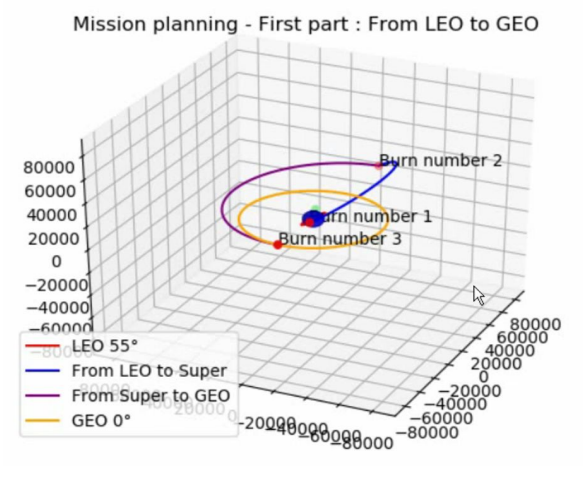
\includegraphics[width=0.6\linewidth]{mission1}
	\caption{Mission planning - First part}
\end{figure}
\textbf{\underline{Phase 2}} :
\begin{itemize}
	\item $\Delta v = 1.57$ km/s
\end{itemize}
{\underline{Further secondary burns}} :
\begin{itemize}
	\item Steering, rotation : $\approx 80$ m/s
	\item Reserve, correction : $\approx 200$ m/s
	\item Capture : $\approx 100$ m/s
\end{itemize}
\underline{\textbf{Total $\Delta v$ for the whole mission}} : $6.61$ km/s
{\underline{Phase 2 savings}} :
\begin{itemize}
	\item Aerobrake : $\approx 390$ m/s
	\item Inclination change during aerobrake : $1470$ m/s
\end{itemize}
\underline{\textbf{Total savings in both phases}} : $2.95$ km/s\\

\autoref{figtim2} shows the paths of the second part of the mission. Here only one exemplary aerobrake orbit is shown as a simplification.
\begin{figure}[H]
	\centering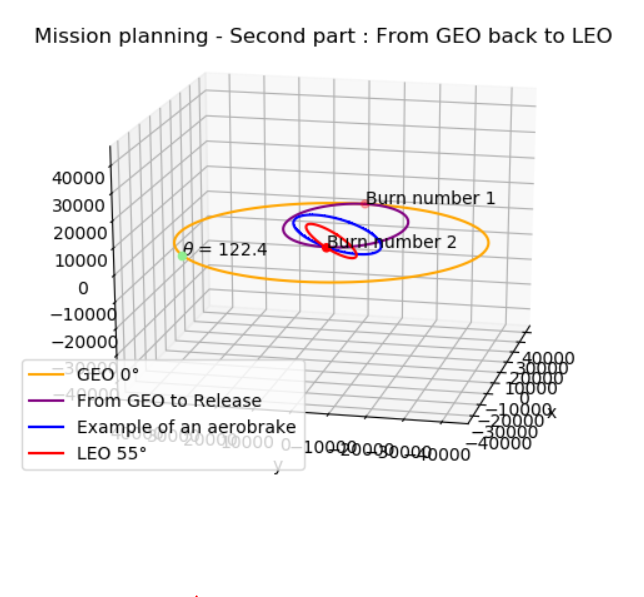
\includegraphics[width=0.7\linewidth]{mission2}
	\caption{Mission planning - Second part}\label{figtim2}
\end{figure}